\chapter{Lezione 4 - Architettura di Enterprise Resource Planning System}

Benvenuti a questa nuova lezione architettura di un enterprise resource planning system.
Tratteremo in questa lezione la parte che riguarda la gestione delle informazioni.
Gli argomenti che tratteremo sono lo schema dell'architettura, i principi fondativi di un enterprise resource planning system e la base delle informazioni, come le informazioni vengono gestite.

Argomenti trattati:

\FloatBarrier
\begin{figure}[H]
  \centering
  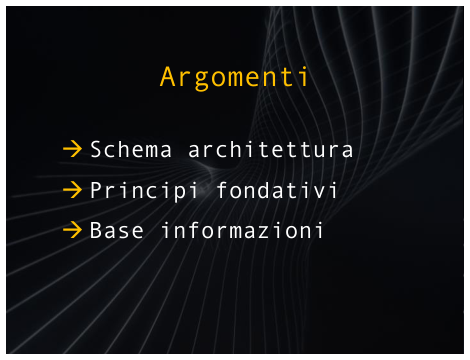
\includegraphics[width=0.50\textwidth,
                    trim=40 100 40 60, % L B R T
                    clip]
                    {images/Lez04_p01_fig_02}
  % \caption{Sommario}
  % \label{fig:Lez15_p06_fig_02}
\end{figure}
\FloatBarrier
\noindent

Ma vediamo innanzitutto il primo argomento, schema dell'architettura, e lo vedremo in una maniera molto sintetica, il massimo della sintesi.

